% Visualisation of Two's complement for a 4-bit-value
% Author: Harald Lichtenstein
\documentclass[tikz,border=10pt]{standalone}
\usetikzlibrary{shadows}  % Used library shadows of the tikz package
\begin{document}
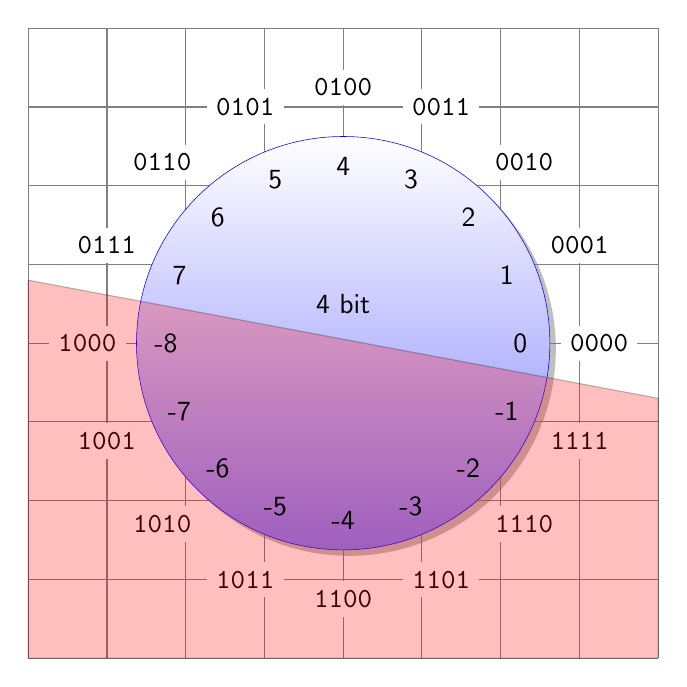
\begin{tikzpicture}[
     auto,                % some style definitions of the elements follow
     node distance = 0cm, % used in this picture
     bin/.style    = {rectangle, fill=white, text=black},
     dec/.style    = {draw=none, text=black},
    circ/.style    = {circle, top color=white, bottom color=blue!50,
    draw=blue, very thin, minimum size=5.25cm, drop shadow={opacity=0.5}}
  ]
  % draw a grid in the background
  \draw[step=1,gray,thin] (-4,-4) grid (4,4);
  \node[circ] (center) at (0,0)  {};
  \node[font=\sffamily]   (4bit)   at (0,.5) {4 bit};

  % Simply hand calculated angles for the positions of the bit values
  %varound the circle

  \foreach \angle / \bits in {%
      0/0000, 22.5/0001, 45/0010, 67.5/0011, 90/0100, 112.5/0101,
    135/0110, 157.5/0111, 180/1000, 202.5/1001, 225/1010, 247.5/1011,
    270/1100, 292.5/1101, 315/1110, 337.5/1111}
    \draw (\angle:3.25cm) node [bin, font=\ttfamily] {\bits};

  \draw[fill=red, opacity=.25]
    (-4,-4) -- (-4cm,.8cm) -- (4cm,-0.7cm) -- (4cm,-4cm) -- cycle;

  % Simply hand calculated angles for the positions of
  % the decimal values around the circle

  \foreach \angle / \dez in {%
    0/0, 22.5/1, 45/2, 67.5/3, 90/4, 112.5/5, 135/6, 157.5/7, 180/-8,
    202.5/-7, 225/-6, 247.5/-5, 270/-4, 292.5/-3, 315/-2, 337.5/-1}
    \draw (\angle:2.25cm) node [dec, font=\sffamily] {\dez};


\end{tikzpicture}
\end{document}
